\chapter{ESP MESH}
        \espmesh\ est le protocole du constructeur Espressif permettant d'établir un réseau mesh avec des \esp.
        Cette section explique le fonctionnement de ce protocole. \espmesh\ a pour objectif la création d'un arbre recouvrant.
        Il existe plusieurs types de noeuds:
        \begin{enumerate}
            \item \textbf{Racine}: seule interface entre le réseau \espmesh\ et un réseau \textsc{ip} externe.
            \item \textbf{Noeuds intermédiaires}: noeuds qui ont un parent et au moins un enfant.
            Ils transmettent leurs paquets et ceux de leurs enfants.
            \item \textbf{Feuilles}: noeuds qui n'ont pas d'enfants et ne transmettent que leurs paquets.
            \item \textbf{Noeuds idle}: noeuds qui n'ont pas encore rejoint un réseau \espmesh.
        \end{enumerate}

        \begin{figure}[H]
            \centering
            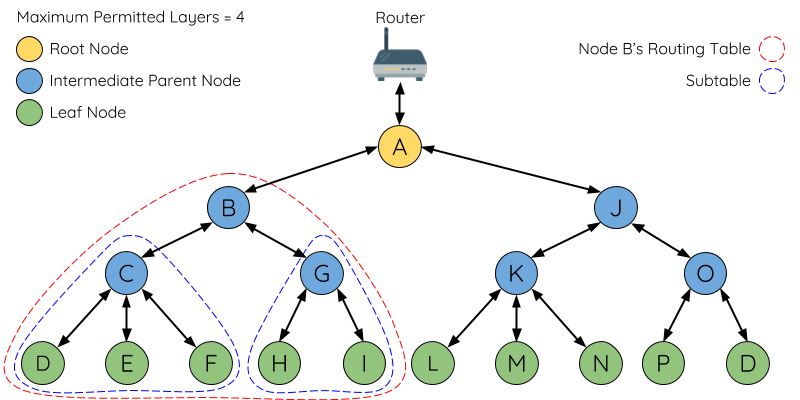
\includegraphics[scale=0.3]{images/mesh-node-types.png}
            \caption{Topologie d'un réseau \espmesh \cite{esp-mesh_w}}
        \end{figure}

        \textbf{Routage}\newline
        \begin{itemize}
            \item Table de routage\\
                Chaque noeud possède sa table de routage. Soit $p$ un noeud, sa table de routage contient les adresses \mac\ 
                des noeuds du sous-arbre ayant $p$ comme racine, et également celle de $p$.\\
                Elle est partitionnée en sous-tables qui correspondent aux sous-arbres des enfants de $p$.
            \item Acheminement de paquets\\
                Quand un paquet est reçu,
                \begin{itemize}
                    \item Si l'adresse \mac\ du paquet est dans la table de routage et si elle est différente de l'adresse du noeud l'ayant reçu, le paquet est envoyé
                    à l'enfant correspondant à la sous-table contenant l'adresse.
                    \item Si l'adresse n'est pas dans la table de routage, le paquet est envoyé au parent.
                \end{itemize}
                %\espmesh\ utilise un mécanisme de vérification de chemin pour détecter les boucles. Si une boucle arrive, un parent va prévenir son enfant et initier une déconnexion.

        \end{itemize}
        \vspace{0.5cm}

        \textbf{Construction d'un réseau}
        \newline
        \begin{enumerate}
            \item \'Election de la racine
                \begin{itemize}
                    \item \textbf{Sélection automatique}\\
                        Chaque noeud idle va transmettre son adresse \mac\ et
                        la valeur de son \rssi\ (Received Signal Strength Indication) avec le routeur via des beacons.
                        Dans le but de choisir comme racine, le noeud le plus proche de l'AP.\\
                        Simultanément, chaque noeud scanne les beacons des autres noeuds. Si un noeud
                        en détecte un autre avec un \rssi\ strictement plus fort, il va transmettre le contenu de
                        ce beacon (càd voter pour ce noeud).\\
                        Ce processus sera répété pendant un nombre minimum d'itérations.\\
                        Après toutes les itérations, chaque noeud va calculer le ratio
                        \[\frac{nombre\ de\ votes}{nombre\ de\ noeuds\ participants\ \textrm{\textit{à l'élection}}}\]
                        Si ce ratio est au-dessus d'un certain seuil (par défaut 90\%), ce noeud deviendra la racine.\footnote{
                            Si plusieurs racines sont élues, deux réseaux \espmesh\ seront créés.
                            Dans ce cas, \espmesh\ possède un mécanisme interne qui va fusionner les deux réseaux
                            ssi les racines sont connectées au même routeur.
                        }



                    \item \textbf{Sélection par l'utilisateur}\\
                        La racine se connecte au routeur et elle, ainsi que les autres noeuds, oublient le processus
                        d'élection.
                \end{itemize}
            \item Formation de la deuxième couche\\
                Une fois le processus d'élection d'une racine terminé, chaque noeud va émettre des beacons
                pour permettre aux autres noeuds de détecter sa présence et de connaître son statut.
                Ces beacons contiennent les informations suivantes:
                \begin{itemize}
                    \item[$\bullet$] Type du noeud (racine, intermédiaire, feuille, idle)
                    \item[$\bullet$] Couche sur laquelle se trouve le noeud
                    \item[$\bullet$] Nombre de couches maximum autorisées dans le réseau
                    \item[$\bullet$] Nombre de noeuds enfants
                    \item[$\bullet$] Nombre maximum d'enfants   
                \end{itemize}
                Les noeuds idle à portée de la racine vont s'y connecter et devenir des noeuds intermédiaires.
            
            \item Formation des autres couches\\
                Les noeuds idle à portée de noeuds intermédiaires vont s'y connecter. Si plusieurs parents
                sont possibles, un noeud choisira son parent selon deux critères connus par les beacons des noeuds intermédiaires.
                \begin{enumerate}
                    \addtolength{\itemindent}{1cm}
                    \item[1.] La couche sur laquelle se situe le candidat parent:
                        le candidat se trouvant sur la couche la moins profonde sera choisi. 
                    \item[2.] Le nombre d'enfants du candidat parent: si plusieurs candidats se trouvent
                        sur la couche la moins profonde, celui avec le moins d'enfants sera choisi. 
                \end{enumerate}
                
                Un noeud peut aussi se connecter à un parent prédéfini.\\

                Une fois connectés, les noeuds deviennent des noeuds intermédiaires si le nombre maximal de couches n'est pas atteint.
                Sinon, les noeuds de la dernière couche deviennent automatiquement
                des feuilles, empêchant d'autres noeuds dans l'état idle de s'y connecter.

        \end{enumerate}
        Pour éviter les boucles, un noeud ne va pas se connecter à un noeud dont l'adresse \mac\ se trouve dans sa table de routage.
        \vspace{0.5cm}

        \textbf{Mise sous tension asynchrone}\newline
            La structure du réseau peut être affectée par l'ordre dans lequel les noeuds sont mis sous tension.
            Les noeuds ayant une mise en tension retardée suivront les deux règles suivantes:
            \begin{enumerate}
                \item Si une racine existe déjà, le noeud ne vas pas essayer d'élire une nouvelle racine
                    même si son \rssi\ avec le routeur est meilleur. Il va rejoindre le réseau comme un noeud idle. \\
                    Si le noeud est la racine désignée, tous les autres noeuds vont rester idle
                    jusqu'à ce que le noeud soit mis sous tension.
                \item Si le noeud devient un noeud intermédiraire, il peut devenir le meilleur parent d'un autre noeud ( cet autre noeud changera donc de parent).
                \item Si un noeud idle a un parent prédéfini et que ce noeud n'est pas sous tension, il ne va pas essayer de se connecter à un autre parent.
            \end{enumerate}
        \vspace{0.5cm}
        \textbf{Défaillance d'un noeud}\newline
            \begin{itemize}
                \item Défaillance de la racine\\
                    Si la racine tombe, les noeuds de la deuxième couche vont d'abord tenter de s'y reconnecter.
                    Après plusieurs échecs, les noeuds de la deuxième couche vont entamer entre eux le processus d'élection d'une nouvelle racine.\\
                    Si la racine ainsi que plusieurs couches tombent, le processus d'élection sera initialisé sur la couche la plus haute.


                \item Défaillance d'un noeud intermédiaire\\
                    Si un noeud intermédiaire tombe, ses enfants vont d'abord tenter de s'y reconnecter.
                    Après plusieurs échecs, ils se connecteront au meilleur parent disponible.\\
                    S'il n'y a aucun parent possible, ils se mettront dans l'état idle.
                    \begin{figure}[H]
                        \centering
                        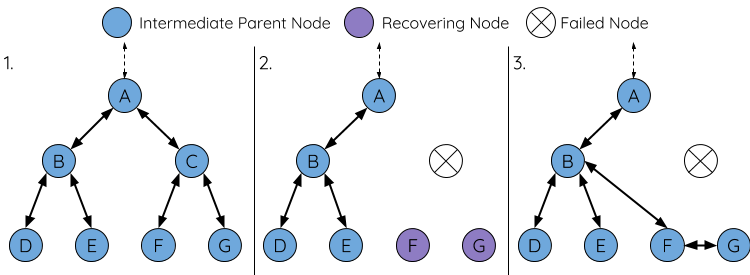
\includegraphics[scale=0.5]{images/mesh-parent-node-failure.png}
                        \caption{Défaillance d'un noeud intermédiaire\cite{esp-mesh_w}}
                    \end{figure}
            \end{itemize}
            \vspace{0.5cm}
            \textbf{Changement de racine}\newline
                Un changement de racine n'est possible que dans deux situations:
                \begin{enumerate}
                    \item La racine tombe. (voir point précédent)
                    \item La racine le demande.
                        Dans ce cas, un processus d'élection de racine sera initialisé. La nouvelle racine élue
                        enverra alors une \textit{switch request} à la racine actuelle qui répondra par un acquittement.
                        Ensuite la nouvelle racine se déconnectera de son parent et se connectera au routeur.
                        L'ancienne racine se déconnectera du routeur et deviendra un noeud idle pour enfin se connecter à un nouveau parent.
                \end{enumerate}
        \textbf{Paquets ESP-MESH}\\
            Les paquets \espmesh\ sont contenus dans une trame WiFi. Une transmission multi-sauts utilisera un paquet \espmesh\ transporté 
            entre chaque noeud par un paquet wifi différent.\\
            La figure \ref{fig_meshPacket} montre la structure d'un paquet \espmesh:\\

            \begin{figure}[h]
                \centering
                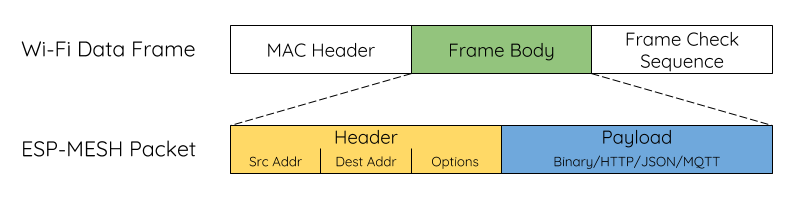
\includegraphics[scale=0.5]{images/mesh-packet.png}
                \caption{Paquet \espmesh\ \cite{esp-mesh_w}}
                \label{fig_meshPacket}
            \end{figure}
            Le header d'un paquet \espmesh\ contient les adresses \mac\ source et destination ainsi que diverses options.\\
            Le payload d'un paquet \espmesh\ contient les données de l'application.
        
        \vspace{0.5cm}
        \textbf{Multicasting}\\
            Le multicasting permet d'envoyer simultanément un paquet \espmesh\ à plusieurs noeuds du réseau. Le multicasting
            peut être réalisé en spécifiant
            \begin{itemize}
                \item Soit un ensemble d'adresses \mac\\
                    Dans ce cas, l'adresse de destination doit être
                    {\fontfamily{qcr}\selectfont \textls[-300]{\small 0 1 : 0 0 : 5 E : x x : x x : x x}}
                    Cela signifie que le paquet est un paquet multicast et que la liste des adresses peut être obtenue dans les options du header.
                \item Soit un groupe préconfiguré de noeuds\\
                    Dans ce cas, l'adresse de destination du paquet doit être l'ID\footnote{Dans un réseau\espmesh, chaque groupe a un ID unique}
                    du groupe et un flag \textsc{mesh\_data\_group} doit être ajouté. % todo ajouté où ?
                    % todo comment les noeuds sont au courant qu'ils sont dans ce groupe
            \end{itemize}

        \vspace{0.5cm}
        \textbf{Broadcasting}\\
            Le broadcasting permet de transmettre un paquet \espmesh\ à tous les noeuds du réseau. Pour éviter de gaspiller de
            la bande passante, \espmesh\ utilise les règles suivantes:
            \begin{enumerate}
                \item Quand un noeud intermédiare reçoit un paquet broadcast de son parent, il va le transmettre à tous ses enfants
                    et en stocker une copie
                \item Quand un noeud intermédiaire est la source d'un paquet broadcast, il va le transmettre à son parent et à ses enfants
                \item Quand un noeud intermédiaire reçoit un paquet d'un de ses enfants, il va le transmettre à ses autres enfants, son parent
                    et en stocker une copie
                \item Quand une feuille est la source d'un paquet broadcast, elle va le transmettre à son parent
                \item Quand la racine est la source d'un paquet broadcast, elle va le transmettre à ses enfants
                \item Quand la racine reçoit un paquet broadcast de l'un de ses enfants, elle va le transmettre à ses autres enfants et en stocker une copie
                \item Quand un noeud reçoit un paquet broadcast avec son adresse \mac\ comme adresse source, il l'ignore
                \item Quand un noeud intermédiaire reçoit un paquet broadcast de son parent, s'il possède une copie de ce paquet (càd que ce paquet a été à l'origine transmis par l'un de ses enfants), il va l'ignorer
                    pour éviter les cycles ( protocole d'inondation)
            \end{enumerate}
        \vspace{0.5cm}
        \textbf{Contrôle de flux}\\%todo pas clair
            Pour éviter que les parents soient submergés de flux venant de leurs enfants, chaque parent va
            assigner une fenêtre de réception à chaque enfant. Chaque noeud enfant doit demander une fenêtre
            de réception avant chaque transmission. La taille de la fenêtre peut être ajustée dynamiquement.
            Une transmission d'un enfant vers un parent se déroule en plusieurs étapes:
            \begin{enumerate}
                \item Le noeud enfant envoit à son parent une requête de fenêtre. Cette requête contient le numéro de séquence du paquet en attente d'envoi.
                \item Le parent reçoit la requête et compare le numéro de séquence avec celui du précédent paquet envoyé par l'enfant.
                    La comparaison est utilisée pour calculer la taille de la fenêtre qui est transmise à l'enfant.
                \item L'enfant transmet le paquet en accord avec la taille de fenêtre. Une fois la fenêtre de réception utilisée, l'enfant doit renvoyer une demande de fenêtre.
            \end{enumerate}
        \vspace{0.5cm}
        \textbf{Performances}\\
            Espressif fournit les performances d'\espmesh\ pour un réseau de 100 noeuds avec un nombre maximum de couches de 6 
            et un nombre d'enfants maximum par noeuds de 6.(voir table \ref{performances_espMesh})
            \begin{table}[H]
                \begin{tabular}{|l|l|}
                    \hline
                    Temps de construction du réseau & $<$ 60 secondes\\ \hline
                    Latence par saut & 10 à 30 millisecondes\\ \hline
                    Temps de réparation du réseau & \makecell{Si la racine tombe: $<$ 10 secondes \\ Si un noeud enfant tombe: $<$ 5 secondes}\\ \hline
                \end{tabular}
                \caption{Performances d'\espmesh\ \cite{esp-mesh_w}}
                \label{performances_espMesh}
            \end{table}

            
        \textbf{Discussion}\\
            A première vue, une topologie en arbre n'est pas robuste car si la racine tombe,
            tout le reste du réseau est déconnecté. Cependant le processus d'élection
            d'une nouvelle racine semble efficace selon les résulats fournis par Espressif.
            Un point négatif du protocole est que pour un noeud donné, sa table de routage contient tous les
            noeuds de son sous-arbre.
            On imagine donc difficilement utiliser ce protocole pour un nombre élevé de noeuds.